\input devHead.tex
\SetTheme{AnnArbor} %11
\title{ソフトウェア開発\\第13回目授業}
\author{平野 照比古}
\institute{}
\date{2018/1/11}
\newtheorem{Prob}{解説}
\newcommand{\Elm}[1]{\texttt{<#1>}}
\setbeamercovered{transparent}

\newcommand{\DOMM}{\texttt}
\newcommand{\Event}{\texttt}
\newcommand{\DOMP}{\texttt}
\newcommand{\DOM}{\texttt{DOM}}
\newcommand{\keyitem}{\relax}
\newcommand{\HTML}{HTML文書}
\begin{document}
\frame{\maketitle}
\section{クラスの例}
 \begin{frame}[containsverbatim]
  \frametitle{例の概要}
\begin{figure}[ht]
 \begin{center}
  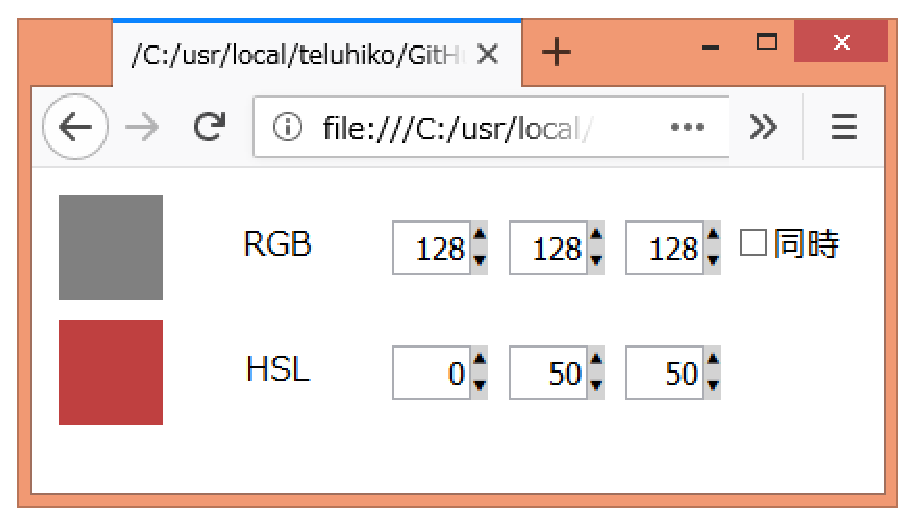
\includegraphics[width=0.5\textwidth]{../13Ex.eps}
 \end{center}
 \caption{色の指定を見る}\label{color}
 \begin{itemize}
  \item 上下2行のテキストボックスで指定された色を左側の正方形の部分で表
        示
  \item 上はRGB形式で、下はHSL\footnote{CSS Color Module Level
3 \texttt{https://www.w3.org/TR/2011/REC-css3-color-20110607/}を参照}形式で色を指定
 \end{itemize}
\end{figure}
 \end{frame}
 \begin{frame}[containsverbatim]
  \frametitle{色を変える操作}
  \begin{itemize}
   \item れぞれのテキストボックスの値は▲をクリックすると増加し、▼をクリッ
       クすると1ずつ減少
   \item シフトキーを押しながらクリックすると5ずつ変化
   \item RGB形式の値は$0\sim255$の間で変化する。上限または下限の範囲を超え
       る場合は上限または下限の値にのままで一番右のチェックボックスを
       チェックすると3つの値が同時に増減
   \item HSL形式の値は一番左(H--色相)が$0\sim359$の間で循環して変化し、残
       りの2つは$0\sim100$の間で変化
  \end{itemize}
 \end{frame}
\section{ソースコードの解説}
\subsection{HTMLファイル}
 \begin{frame}[containsverbatim]
  \frametitle{HTMLファイルのソース}
\LISTN{13Ex.html}{1}{last}{\footnotesize}
 \end{frame}
 \begin{frame}[containsverbatim]
  \frametitle{HTMLファイルのソース--解説}
\begin{itemize}
 \item 5行目ではこのページに関する処理を定義する JavaScript ファイル
       (\texttt{13Ex.js})を読み込む。
 \item 6行目ではユーザーインターフェイスを定義しているJavaScript ファイル
       (\texttt{13UI.js})を読み込む。
 \item 7行目から15行目は色を表示する部分のCSSを定義している。
       \begin{itemize}
        \item 9行目と10行目では表示部分の大きさ
        \item 11行目では配置方法(横に並べる)
        \item 12行目では上下の位置(ここでは中央に指定)
        \item 13行目では色の表示域の周りの空白
       \end{itemize}
 \item 18行目と19行目では色の表示位置と値を設定するための\texttt{<div>}
       要素を定義
\end{itemize}
 \end{frame}
 \section{ユーザーインターフェイス}
 \begin{frame}[containsverbatim]
  \frametitle{オブジェクトのオプションの値を変更する関数}
 \LISTN{13UI.js}{1}{5}{\footnotesize}
\begin{itemize}
 \item 2番目の引数(\texttt{Opt})は変更する値が入っているオブジェクト
 \item 1番目の引数はキーがオブジェクト内の指定できるオプション(デフォル
       ト値が設定されている)からなるオブジェクト
 \item 3行目で指定できるキーであれば値を設定
\end{itemize}
 \end{frame}
 \begin{frame}[containsverbatim]
  \frametitle{TML要素の\texttt{style}を設定する関数}
\LISTN{13UI.js}{6}{9}{\footnotesize}
\begin{itemize}
 \item 7行目で、指定されたオプションを設定
 \item 9行目でオプションのオブジェことを\texttt{style}属性の形式になるよ
       うに変更
\begin{enumerate}
 \item オブジェクトを\texttt{JSON}形式の文字列に変換
 \item キーなどを囲む\texttt{\{}と\texttt{"}を取り除く%"
 \item \texttt{,}と\texttt{\}}を\texttt{;}に変換
\end{enumerate}
\end{itemize}
 \end{frame}
 \begin{frame}[containsverbatim]
  \frametitle{基本となるオブジェクト\texttt{DOMObject}(1)}
\LISTN{13UI.js}{10}{15}{\footnotesize}
\begin{itemize}
 \item オブジェクト内で有効な定数を定義するためにクラス式を返す関数を定
       義しその場で実行している(35行目の\texttt{()})。
 \item 11行目から14行目で作成する要素の名前空間のリストをオブジェクトリ
       テラルの形で定義。ここではHTML要素とSVG要素の名前空間があ
       る。
\end{itemize}
 \end{frame}
 \begin{frame}[containsverbatim]
  \frametitle{基本となるオブジェクト\texttt{DOMObject}(2)}
\LISTN{13UI.js}{16}{23}{\footnotesize}
 \end{frame}
 \begin{frame}[containsverbatim]
  \frametitle{基本となるオブジェクト\texttt{DOMObject}--解説(2)}
\begin{itemize}
 \item 16行目から18行目で\texttt{document.getElementById()}に相当するこ
       のオブジェクト用の関数を定義
 \item 19行目から23行目で\texttt{document.getElementsByTagName()}の相当する
       このオブジェクト用の関数を定義
       \begin{itemize}
        \item 20行目で指定された要素のリストを得ている。
        \item 21行目から22行目でそのリストを\texttt{DOMObject}のリストに
              変更
        \item \ElmJ{map}は配列オブジェクト\ElmJ{Array}のメソッドで、各要
              素に対して引数で与えられた関数を実行し、その結果からなる配
              列を返す。
        \item 20行目で得たリストは配列ではないのでこのメソッドを使用不可
        \item \ElmJ{call}は指定した関数が参照する\ElmJ{this}をその1番目
              の引数にする。
        \item 22行目の\texttt{(E)}以降の書き方は新しい無名関数の
              記述方法。\Verb+function(E){...}+と書くのと同じ。
       \end{itemize}
\end{itemize}
 \end{frame}
 \begin{frame}[containsverbatim]
  \frametitle{基本となるオブジェクト\texttt{DOMObject}--解説(2 続き)}
\begin{itemize}
        \item 新しい記述一番の違いは関数内での
              \ElmJ{this}の取り扱い。
        \item \ElmJ{class}内のコードは\texttt{strict}モードで実行
        \item \ElmJ{function}で定義された関数内では\ElmJ{this}は
              \ElmJ{undefined}
        \item 簡略化された記述では\ElmJ{this}の値がオブジェクト自身
        \item この違いが問題となる例はこのリストの141行目などにある。
\end{itemize}
 \end{frame}
 \begin{frame}[containsverbatim]
  \frametitle{基本となるオブジェクト\texttt{DOMObject}(3)}
\LISTN{13UI.js}{24}{31}{\footnotesize}
 \end{frame}
 \begin{frame}[containsverbatim]
  \frametitle{基本となるオブジェクト\texttt{DOMObject}--解説(3)}
 24行目から31行目はこのオブジェクトの\ElmJ{constructor}を定義して
       いる。
       \begin{itemize}
        \item 引数は順に作成する要素名、その属性のリスト、親要素、イベン
              ト処理のリスト、名前空間(デフォルトはHTML)
        \item 26行目で名前空間を指定して要素を作成
        \item 27行目は作成した要素に、与えられた属性を設定する関数を呼び
              出している。
        \item 28行目では親要素がある場合にはその子要素になるよ
              うに指定
        \item 29行目ではイベント処理を設定
        \item 32行目から34行目では与えられたリストの属性を設定する関数を
              定義
       \end{itemize}
 \end{frame}
 \begin{frame}[containsverbatim]
  \frametitle{与えられた文字列を表示するためのクラス\texttt{divWithText}}
\LISTN{13UI.js}{36}{41}{\footnotesize}
\begin{itemize}
 \item このクラスは\texttt{DOMObject}を継承
 \item コンストラクタの引数は順に、表示するテキスト、親要素、属性の3つ
 \item 39行目で\texttt{<div>}要素を作成し、その要素の\ElmJ{innerText}プロパティを
       設定することで表示を可能としている
\end{itemize}
 \end{frame}
 \begin{frame}[containsverbatim]
  \frametitle{\texttt{SpinBox}のクラス--\texttt{constructor}(1)}
HTMLにも\texttt{spinbox}があるが少し機能を変えている。

  このクラスのコンストラクタの部分である。
  \LISTN{13UI.js}{42}{49}{\footnotesize}
 \end{frame}
 \begin{frame}[containsverbatim]
  \frametitle{\texttt{spinbox}クラス--\texttt{constructor}解説(1)}
\begin{itemize}
 \item コンストラクタの引数は順に、オプション、親要素、イベント処理関数
       群、値が変化したときの処理関数
 \item 44行目は値が変化したときに呼び出される関数をオブジェクトに登録
 \item 45行目から49行目ではこのオブジェクトのデフォルトのパラメータを定
       義
       \begin{itemize}
        \item \texttt{max}は設定できる値の最大値(デフォルト値は
              JavaScriptで扱うことができる最大値)
        \item \texttt{mix}は設定できる値の最小値(デフォルト値は
              JavaScriptで扱うことができる最小値)
        \item \texttt{skip}は値の変化量(デフォルト値は$1$)
        \item \texttt{bigSkip}はシフトキーを押しながらクリックしたときの
              値の変化量(デフォルト値は$5$)
        \item \texttt{value}は初期値(デフォルト値は$0$)
        \item \texttt{type}は両端の値から外れたときの処理方法(デフォルト
              は両端の値に固定--\texttt{"limited"}。値が循環的に変わる
              \texttt{"cyclic"}がある)
       \end{itemize}
\end{itemize}
 \end{frame}
 \begin{frame}[containsverbatim]
  \frametitle{\texttt{SpinBox}のクラス--\texttt{constructor}(2)}
  \LISTN{13UI.js}{50}{55}{\footnotesize}
 \begin{itemize}
  \item 50でオブジェクトの周りの余白の設定
  \item 51行目で入れ物の\texttt{<div>}要素を作成
 \item 52行目では45行目からのデフォルトのパラメータを与えられた値に変更
 \item 53行目から55行目では56行目から58行目で定義されるテキストボックス
       を入れるための\texttt{<div>}要素を作成
 \end{itemize}
 \end{frame}
 \begin{frame}[containsverbatim]
  \frametitle{\texttt{SpinBox}のクラス--\texttt{constructor}(2)}
  \LISTN{13UI.js}{56}{73}{\footnotesize}
 \end{frame}
 \begin{frame}[containsverbatim]
  \frametitle{\texttt{spinbox}クラス--解説(2)}
\begin{itemize}
 \item 56行目から58行目で定義されるテキストボックスは値を直接変更できな
       い設定をしている(\texttt{"readonly"}の指定)
 \item 59行目から60行目ではテキストボックスの隣に置く上下のボタンを入れ
       るための\texttt{<div>}要素を作成
 \item 61行目から64行目では値の上下させるボタンの表示形式を定義
 \item 65行目でさらにボタンのタイプ(値を増加)を設定し、66行目から67行目でボタンと
       して機能するようなオブジェクトを追加。この上でクリックイ
       ベントが生じたときにイベント発生時ののシフトキーの状態を
       \texttt{sipnbox}の\texttt{up}プロパティの与えている(代入で行って
       いるが、\texttt{up}は76行目から85行目で定義されているセッターで
       ある)。
 \item 69行目から72行目は値を減少させるボタンを設定
\end{itemize}
 \end{frame}
 \begin{frame}[containsverbatim]
  \frametitle{セッターとゲッターを定義(1)--値の増加の処理}
\LISTN{13UI.js}{74}{85}{\footnotesize}
 \end{frame}
 \begin{frame}[containsverbatim]
  \frametitle{セッターとゲッターを定義--解説}
\begin{itemize}
 \item 74行目と75行目はそれぞれテキストボックスの値に関するゲッ
       ターとセッター
 \item 76行目から85行目は設定値を増大させるメソッドであり、86行目から
       95行目は設定値を減少させるメソッド
 \item 77行目ではシフトキーが押されているかを判定して、変化量を決定
 \item 78行目で仮の値を求め、それが上限値を超えている処理を79行目から
			 83行目で行っている。
 \item
			 上限値で固定(\texttt{type}が\texttt{"limited"})のときは
       上限値と仮の値の小さい方を設定(80行目)。
\item		値が循環する(\texttt{type}が\texttt{"cyclic"})ときは
       上限値が超えた場合、上限値の値を引いている821行目)。
 \item 値の設定後の処理関数が定義されているときはその関数を呼び出す(84
       行目)。
\end{itemize}
 \end{frame}
 \begin{frame}[containsverbatim]
  \frametitle{セッターとゲッターを定義--値の減少の処理}
\LISTN{13UI.js}{85}{96}{\footnotesize}
  値が減少する場合も同様
 \end{frame}
 \begin{frame}[containsverbatim]
  \frametitle{色の3成分を設定するクラス(1)}
\LISTN{13UI.js}{97}{104}{\footnotesize}
 \begin{itemize}
 \item コンストラクタに引数は順に、左端に示すテキスト、RGB形式かHSL形式
			 のタイプ、親要素、値が変化したときの処理関数、オブジェクトのオプ
			 ションである。
 \item 99行目のコメント行は、メソッド内で呼び出される無名関数内でオブ
			 ジェクト自身を示す\ElmJ{this}が参照できないときの対処法である。
			 \ElmJ{this}を変数(\texttt{that})に格納し、それを参照する。
 \item 110行目から104行目は左端にテキストが表示されるようにしている。
 \end{itemize}
 \end{frame}
 \begin{frame}[containsverbatim]
  \frametitle{色の3成分を設定するクラス(2)}
\LISTN{13UI.js}{105}{116}{\footnotesize}
\end{frame}
 \begin{frame}[containsverbatim]
  \frametitle{色の3成分を設定するクラス--タイプ\texttt{"rgb"}解説(1)}
			 \begin{itemize}
				\item 106行目でタイプを\texttt{"rgb"}に設定
				\item 107行目から116行目でオブジェクト全体を囲む要素を作成して、
							そこに\texttt{click}イベントの処理関数を定義
				\item 右端のチェックボックスにチェックがあ
							る場合はRGBの値を一斉に増減。そのときは(109行目)この関
							数で処理(110行目から112行目)。
				\item 110行目から111行目でRGBの値を変化(\texttt{this.RGB.forEach})。
				\item それぞれの\texttt{sipnbox}にもイベントの処理関数がついてい
							るので、2回処理させないために、112行目でイベントの伝搬を止
							める(\texttt{E.stopPropagation()})。
				\item その後、登録された処理関数を呼び出している。
			 \end{itemize}
 \end{frame}
 \begin{frame}[containsverbatim]
  \frametitle{色の3成分を設定するクラス--タイプ\texttt{"rgb"}(2)}
\LISTN{13UI.js}{117}{128}{\footnotesize}
\end{frame}
 \begin{frame}[containsverbatim]
  \frametitle{色の3成分を設定するクラス--タイプ\texttt{"rgb"}解説(2)}
			 \begin{itemize}
			  \item 126行目から133行目では\texttt{spinbox}3つ作成のために、
							大きさ3の配列を作成し(\texttt{new Array(3)})、それぞれに
							\texttt{0}を設定(\texttt{fill(0)})する。この配列に
							\texttt{forEach}を用いて\texttt{spinbox}を作成

							\ElmJ{Array}のメソッド\ElmJ{forEach}は\ElmJ{undefined}の要
							素に対して実行されないのでこのような処理が必要となる。
				\item これらの\texttt{spinbox}はタイプが\texttt{"limited"}、
							最小値が\texttt{0}、最大値が\texttt{255}、初期値を
							\texttt{128}である。
				\item 134行目から136行目ではRGB値を同時に変化させるかどうかのチェッ
							クボックスを作成
			 \end{itemize}
 \end{frame}
 \begin{frame}[containsverbatim]
  \frametitle{色の3成分を設定するクラス--タイプ\texttt{"rgb"}(2)}
\LISTN{13UI.js}{129}{139}{\footnotesize}
\end{frame}
 \begin{frame}[containsverbatim]
  \frametitle{色の3成分を設定するクラス--タイプ\texttt{"hsl"}}
			 \begin{itemize}
				\item 129行目でタイプを\texttt{"hsl"}に設定している。
				\item 130行目ではオブジェクト全体を囲む要素を定義している。
				\item 131行目から1138 目では3つの\texttt{spinbox}を定義している。
				\item 色相(H)と残りの2つでは値の範囲と取り扱いが異なるので、範囲
							と初期値を与える配列を利用して3つの\texttt{spinbox}を作成
							している。
				\item 139行目でははじめの\texttt{spinbox}のタイプを
							\texttt{"cyclic"}に修正している。
			 \end{itemize}
 \end{frame}
 \begin{frame}[containsverbatim]
  \frametitle{色の3成分を設定するクラス(3)}
\LISTN{13UI.js}{140}{last}{\footnotesize}
\end{frame}
 \begin{frame}[containsverbatim]
  \frametitle{色の3成分を設定するクラス(3)--解説}
  \begin{itemize}
 \item 142行目では\texttt{rgb}の値をコピーして配列で返すゲッターを、
 143行目では\texttt{rgb}の値のセッターをを定義している。
 \item 144行目では\texttt{hsl}の値をコピーして配列で返すゲッターを、
 145行目では\texttt{hsl}の値のセッターをを定義している。
 \item 146行目から150行目ではCSS3で定義されているRGBやHSL形式に変換する
			 メソッドを定義している。
\end{itemize}
 \end{frame}
 \section{ユーザーインターフェイスを引用するJavaScriptファイル}
 \begin{frame}[containsverbatim]
  \frametitle{色の変化を見えるようにする}
 \LISTN{13Ex.js}{1}{last}{\footnotesize}
 \end{frame}
 \begin{frame}[containsverbatim]
  \frametitle{色の変化を見えるようにする--(解説)}
 \begin{itemize}
	\item 2行目から6行目までで2つの色が設定できるオブジェクトを作成してい
				る。一つ目はRGB形式で2つ目がHSL形式となる。区別するパラメータは
				配列で与えている。
	\item 7行目ではその値を左側の背景色に反映するための関数を呼び出してい
				る。
	\item 8行目から11行目では\texttt{spinbox}で設定された色を背景色に設定
				する関数である。
	\item 10行目で\texttt{spinbox}の値を文字列に変換することで行っている。
 \end{itemize} \end{frame}
\end{document}
 \begin{frame}[containsverbatim]
  \frametitle{}
 \end{frame}
